%% LaTeX document -- Revisão Bibliográfica
%% Projeto Integrador -- FEUP
%%
%% Autor: Alexandre Ferreira

\documentclass[11pt,a4paper]{article}

%%------------------------------- preamble ------------------------------------

\usepackage[portuges]{babel}
\usepackage[utf8]{inputenc}
\usepackage[T1]{fontenc}
\usepackage{newtxtext,newtxmath}
\usepackage{amsmath}
\usepackage{setspace}
\usepackage{graphicx}
\usepackage[normalem]{ulem}
\usepackage{caption}
\usepackage{float}
\usepackage{subcaption}
\usepackage{booktabs}
\usepackage[table]{xcolor}
\usepackage{xurl}
\usepackage{csquotes}
\usepackage[backend=biber,authordate]{biblatex-chicago}
\usepackage[printonlyused]{acronym}
\usepackage{eurosym}
\usepackage{siunitx}

%% document dimensions
\usepackage[a4paper,left=25mm,right=25mm,top=25mm,bottom=25mm,headheight=6mm,footskip=12mm]{geometry}
\setlength{\parindent}{0em}
\setlength{\parskip}{1ex}

%% headers & footers
\usepackage{lastpage}
\usepackage{fancyhdr}
\fancyhf{}
\rhead{\small{\emph{\projtitle, \projauthor}}}
\rfoot{\small{\thepage\ / \pageref{LastPage}}}
\pagestyle{fancy}
\renewcommand{\headrulewidth}{0.4pt}
\renewcommand{\footrulewidth}{0.4pt}

%% colors
\usepackage{color}
\definecolor{engineering}{rgb}{0.549,0.176,0.098}
\definecolor{cloudwhite}{cmyk}{0,0,0,0.025}

%% hyperreferences
\usepackage{hyperref}
\hypersetup{
    plainpages=false,
    pdfpagelayout=SinglePage,
    bookmarksopen=false,
    bookmarksnumbered=true,
    breaklinks=true,
    linktocpage,
    colorlinks=true,
    linkcolor=engineering,
    urlcolor=engineering,
    filecolor=engineering,
    citecolor=engineering,
    allcolors=engineering
}

%% path to the figures directory
\graphicspath{{../report/figures/}}

%% bibliography file
\addbibresource{bibliography.bib}

%% macros
\newcommand{\school}{Faculdade de Engenharia da Universidade do Porto}
\newcommand{\degree}{Licenciatura em Engenharia Informática e Computação}
\newcommand{\projtitle}{Modelização e Previsão de Ondas Oceânicas com Base em Fusão Multissensorial}
\newcommand{\subtitle}{Revisão Bibliográfica}
\newcommand{\projauthor}{Alexandre Ferreira}
\newcommand{\supervisor}{Prof.\ Eduardo Silva}
\newcommand{\tutor}{Prof.\ Pedro Ribeiro}

%%------------------------------- document ------------------------------------

\begin{document}

\pagenumbering{roman}\setcounter{page}{1}
\pagestyle{plain}

%%------------------------------- cover page ----------------------------------

\begin{titlepage}
\center

\vspace{-15mm}
{\Large \textbf{\textsc{\school}}}\\

\vfill

{\Large \textbf{\projtitle}}\\[8mm]
{\large \textbf{\subtitle}}\\[28mm]

{\Large \textbf{\projauthor}}\\

\vfill


\includegraphics[width=52mm]{uporto-feup.pdf}

\vfill

{\large \textbf{\degree}}\\[8mm]
{\large \textbf{Tutor na U.Porto}: \tutor}\\[2mm]
{\large \textbf{Orientador na empresa}: \supervisor}\\[18mm]

\today

\end{titlepage}

%%------------------------------- table of contents ---------------------------

\renewcommand{\contentsname}{Índice}
\tableofcontents
\cleardoublepage

%%------------------------------- main content --------------------------------

\pagenumbering{arabic}\setcounter{page}{1}
\pagestyle{fancy}

%%------------------------------- 1. Introdução -------------------------------

\section{Introdução}\label{sec:intro}
O presente estágio insere-se no âmbito dos projetos SEAWINGS e AIRSHIP, iniciativas que visam o desenvolvimento de plataformas aéreas autónomas inovadoras, especificamente desenhadas para operação sobre ambientes marítimos. O traço distintivo destas plataformas é a sua conceção como veículos de Efeito de Solo (\textit{Wing-In-Ground} ou WIG). Estes veículos destacam-se pelo requisito operacional de voar a velocidades elevadas e a altitudes extremamente baixas, frequentemente a apenas um ou dois metros acima da superfície da água. Esta configuração de voo  permite tirar partido do fenómeno aerodinâmico do "efeito de solo", criando um colchão de ar sob a estrutura que aumenta drasticamente a sustentação e a eficiência energética do veículo.

\begin{figure}[h]
     \centering
          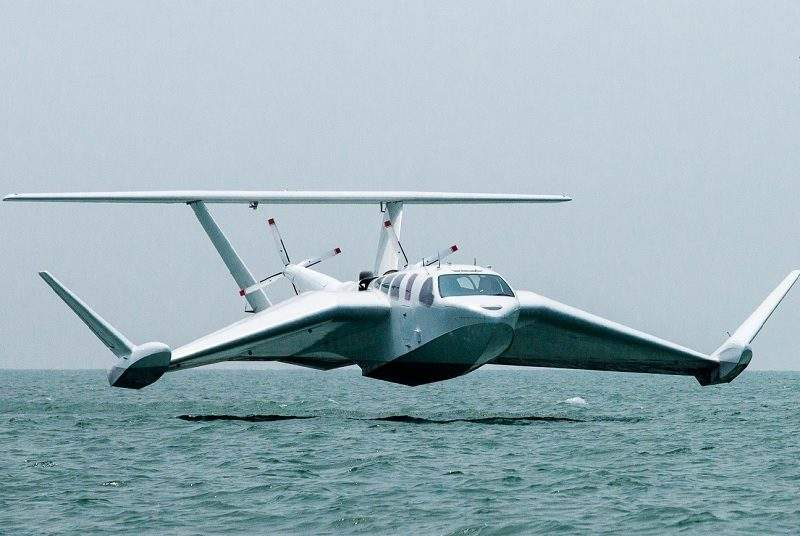
\includegraphics[width=0.7\textwidth]{../imagens/wig.jpg}
     \caption{Exemplo de um veículo a operar sob o princípio do Efeito de Solo (WIG).}
     \label{fig:wig_effect}
 \end{figure}

Devido a este requisito de voo rápido e a baixa altitude, um dos desafios centrais e mais críticos destes projetos é a perceção precisa e em tempo real da superfície do mar. Num ambiente onde a margem para erro é mínima e a dinâmica fluida é imprevisível, a deteção atempada da ocorrência de ondas não é apenas uma questão de mapeamento topográfico, mas sim um requisito fundamental de segurança. A capacidade de "ver" a água à frente do veículo garante que os sistemas de controlo consigam efetuar manobras evasivas ou ajustes de altitude, evitando colisões catastróficas com a ondulação.

As ondas oceânicas constituem um fenómeno dinâmico e periódico, caracterizado principalmente pela sua amplitude, direção e frequência. A correta estimação geométrica e cinemática destes parâmetros, bem como a possibilidade de prever a propagação temporal e espacial das ondas a curto prazo, contribui significativamente para a robustez dos sistemas de controlo e planeamento de trajetória destas plataformas em desenvolvimento.

Neste contexto, o estágio tem como objetivo principal o estudo, desenvolvimento e validação de abordagens de perceção e modelização de ondas oceânicas, baseadas em arquiteturas de fusão multissensorial. No presente relatório, é apresentado o estudo do estado da arte relativo aos modelos hidrodinâmicos e às técnicas de perceção adequadas para dar resposta aos exigentes constrangimentos de operação dos veículos WIG.
No presente relatório, é apresentado o estudo do estado da arte em modelização de ondas e perceção multissensorial. 

%%------------------------------- 2. Modelos de Ondas Oceânicas ---------------

\section{Modelos de Ondas Oceânicas}\label{sec:ondas}

De modo a caracterizar as ondas oceânicas, é fundamental compreender os modelos que descrevem a sua formação e propagação. Estes estabelecem os
parâmetros essenciais para a caracterização de uma onda: a amplitude, comprimento de onda, e a profundidade da água sobre a qual a onda se propaga.

\subsection{Teoria de Ondas Lineares}
A Teoria de Ondas Lineares (ou Teoria de Airy) constitui a aproximação de primeira ordem para o movimento de ondas de superfície. Baseia-se na simplificação das equações de Navier-Stokes, assumindo que o fluido é incompressível e irrotacional, o que permite definir um potencial de velocidade $\phi$ que satisfaz a Equação de Laplace:

\begin{equation}
     \nabla^2 \phi = 0
\end{equation}

Ao aplicar as condições de fronteira na superfície livre (linearizadas) e no fundo do mar, obtemos a expressão da elevação da onda $\eta(x,t)$ \parencite{dean1991water}:

\begin{equation}
     \eta(x,t) = \frac{H}{2}cos(kx - \omega t)
\end{equation}

\begin{figure}[H]
     \centering
          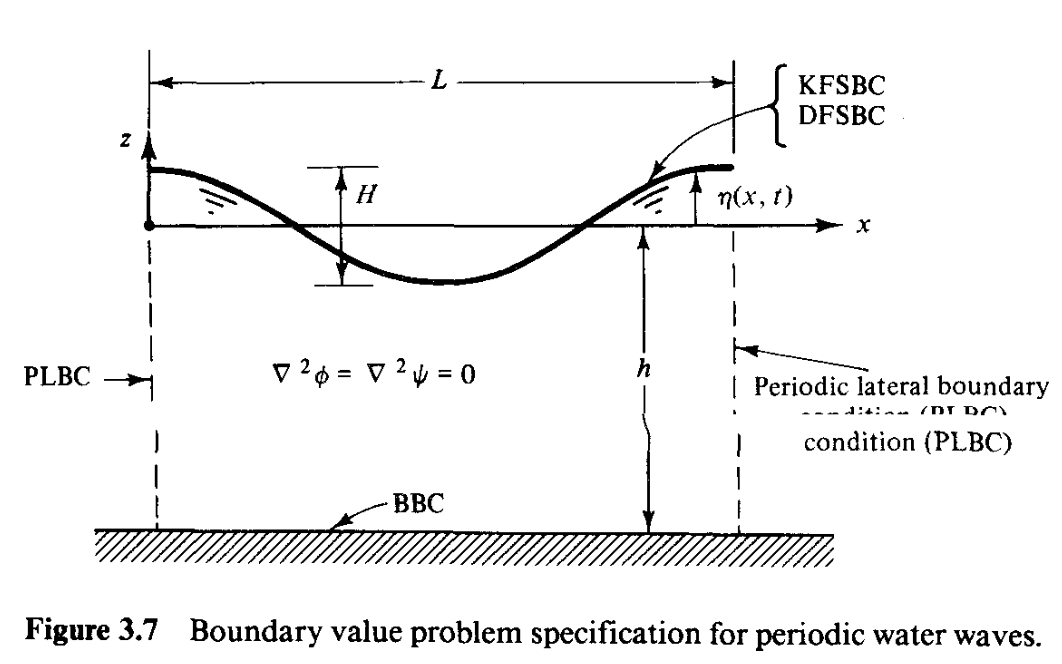
\includegraphics[width=0.7\textwidth]{../imagens/airy_waves.png}
     \caption{Representação gráfica de uma onda linear, ilustrando os parâmetros de onda referidos.}
     \label{fig:airy_waves}
\end{figure}

\subsection{Ondas de Stokes}
Enquanto a teoria linear de Airy assume uma simetria perfeita, a realidade física do mar apresenta cristas mais agudas e vales mais planos. Esta deformação é modelada através da Teoria de Stokes, que expande a elevação da superfície $\eta$ numa série de potências \parencite{dean1991water}.

A elevação total de segunda ordem é a soma da componente linear ($\eta_1$) com uma componente de correção ($\eta_2$) que introduz a assimetria característica das ondas reais:
\begin{equation*}
     \eta = \eta_1 + \eta_2 = \frac{H}{2}\cos(kx - \omega t) + \eta_2
\end{equation*}

A expressão para $\eta_2$ é dada por:
\begin{equation*}
     \eta_2 = \frac{1}{16} \frac{\sinh^3(kh)}{\cosh(kh)} [2 + \cosh(2kh)] \cos(2(kx - \omega t))
\end{equation*}

Esta expansão é fundamental pois os termos hiperbólicos ($\sinh$, $\cosh$) atuam como fatores de escala que dependem da profundidade $h$. Em águas rasas, estes termos amplificam a crista da onda, garantindo que não se subestime a elevação real da superfície. Para o caso simplificado de águas profundas ($kh \to \infty$), a expressão reduz-se à forma mais simples:
\begin{equation*}
     \eta_2 = \frac{1}{2} \frac{k a^2}{\cosh(kh)} \cos(2(kx - \omega t))
\end{equation*}

Para atingir o limite prático de precisão antes da quebra da onda, recorre-se à Quinta Ordem de Stokes. Nesta abordagem, a elevação é descrita por uma soma de cinco termos de Fourier:
\begin{equation*}
     \eta(x,t) = \frac{1}{k} \sum_{n=1}^{5} C_n \cos(n\theta)
\end{equation*}

Nesta ordem superior, a relação de dispersão torna-se também ela não-linear, o que significa que a velocidade de propagação c passa a depender da altura da onda H:
\begin{equation*}
     c^2 = \frac{g k}{\tanh(kh)} [1 + (\frac{k a}{\cosh(kh)})^2 f_1(kh) + (\frac{k a}{\cosh(kh)})^4 f_2(kh)]
\end{equation*}

\subsection{Modelos Estocásticos de Ondas}

Na realidade, a superfície do mar não é composta por uma única onda regular, mas sim pela sobreposição de infinitos componentes com diferentes frequências, amplitudes e direções. Para modelar esta superfície, utiliza-se a Densidade Espectral de Energia S($\omega$), que descreve como a energia das ondas está distribuída por diferentes frequências.

\subsubsection{Espectro de Pierson-Moskowitz}

O modelo de Pierson-Moskowitz \parencite{pierson1964frequency} descreve um mar totalmente desenvolvido, ou seja, um estado em que o vento soprou com velocidade constante por um longo período sobre uma área vasta, e as ondas atingiram o equilíbrio energético com o vento.

A densidade espectral é definida em função da frequência angular $\omega$ e da velocidade do vento $U$ a 19,5 metros de altitude:
\begin{equation*}
     S_{\mathrm{PM}}(\omega)=\alpha g^2 \omega^{-5} \exp\left[-0.74\left(\frac{U\omega}{g}\right)^4\right]
\end{equation*}

Onde:

     $\alpha=8.1\times 10^{-3}$ (Constante de Phillips).

    $g$ é a aceleração da gravidade.

Este espectro fornece a curva esperada do mar em oceano aberto, permitindo a estimativa da altura significativa ($H_s$), que é aproximadamente $4\sqrt{m_0}$, onde $m_0$ é a área sob a curva do espectro.

\subsubsection{Espectro JONSWAP}

O espectro JONSWAP (Joint North Sea Wave Project) \parencite{hasselmann1973measurements} é uma extensão do modelo PM, desenhado para descrever mares em desenvolvimento, onde o fetch (distância sobre a qual o vento sopra) é limitado. Este modelo é caracterizado por um pico de energia muito mais estreito e pronunciado do que o PM.

A formulação do JONSWAP introduz um fator de realce de pico ($\gamma$):
\begin{equation*}
      S_{\mathrm{J}}(\omega)=S_{\mathrm{PM}}(\omega)\,\gamma^{\exp\left[-\frac{(\omega-\omega_p)^2}{2\sigma^2\omega_p^2}\right]}
\end{equation*}

Onde:

     $\gamma$: Fator de realce (tipicamente 3.3).

     $\omega_p$: Frequência de pico (onde a energia é máxima).

     $\sigma$: Parâmetro de largura do pico.
    
Este modelo revela-se mais adequado para descrever as condições de mar em zonas costeiras, onde as ondas ainda não atingiram o equilíbrio energético.

\subsection{Modelos de Águas Rasas (Equações de Boussinesq)}


%%------------------------------- 3. Técnicas de Perceção -----------

\section{Técnicas de Perceção}\label{sec:percecao}
Para realizar a modelação do ambiente marítimo, existem 
diversas técnicas de perceção baseadas em diferentes tipos 
de sensores. Cada uma destas abordagens possui vantagens e 
limitações específicas, as quais determinam a sua 
adequabilidade para o mapeamento e navegação sobre as ondas, 
conforme detalhado de seguida.

\subsection{Radar de Onda Contínua Modulada por Frequência (FMCW)}
Os radares FMCW destacam-se por serem sensores excecionalmente robustos face a condições atmosféricas adversas, operando de forma fiável em cenários onde os sistemas óticos e LiDAR falham. Conseguem manter alcances na ordem das dezenas a centenas de metros em ambientes com chuva, nevoeiro cerrado ou ausência total de iluminação. Distinguem-se também pela capacidade de medir diretamente a velocidade relativa dos objetos com base no efeito Doppler, permitindo o isolamento eficaz de alvos em movimento dinâmico \parencite{11139524}.

No entanto, a utilização de radares FMCW para a modelação geométrica de ondas apresenta desafios significativos. As leituras obtidas destes sensores não consistem em representações topográficas contínuas, mas sim em nuvens de pontos tridimensionais altamente esparsas (\textit{sparse point cloud}) e ruidosas. Ao interagir com a superfície aquática, as micro-ondas sofrem frequentemente reflexão especular, desviando o sinal para longe do recetor. Consequentemente, o radar regista predominantemente os ecos provenientes das cristas das ondas ou de superfícies perpendiculares ao feixe de emissão, deixando vastas áreas da superfície do mar não mapeadas \parencite{10683889}.

\begin{figure}[h]
     \centering
          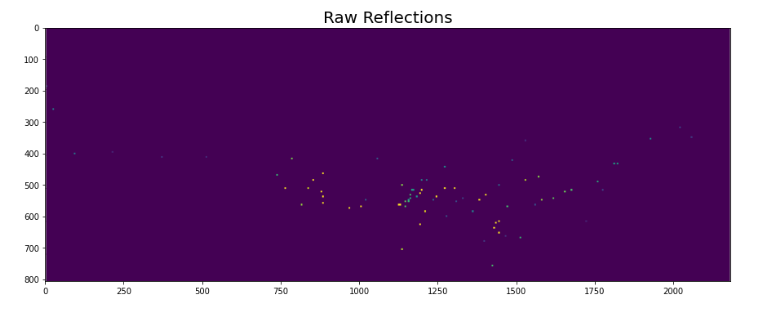
\includegraphics[width=0.7\textwidth]{../imagens/raw_fmcw_radar.png}
     \caption{Exemplo de dados brutos de um radar FMCW.}
     \label{fig:radar_fmcw_raw}
 \end{figure}

Adicionalmente, os radares apresentam uma resolução espacial consideravelmente inferior à dos sensores baseados em luz e são suscetíveis à geração de um elevado volume de deteções falsas (ruído de fundo ou \textit{clutter}) provocado pela dispersão do sinal no \textit{spray} marítimo e por reflexões múltiplas (\textit{multipath}). Devido a estas características intrínsecas dos dados recolhidos, a extração de um modelo tridimensional contínuo das ondas obriga a um elevado esforço de processamento computacional, suportado por complexos algoritmos de filtragem espacial e temporal \parencite{nowak2022weavenet}.

\begin{figure}[h]
     \centering
     \begin{subfigure}[t]{0.49\textwidth}
          \centering
          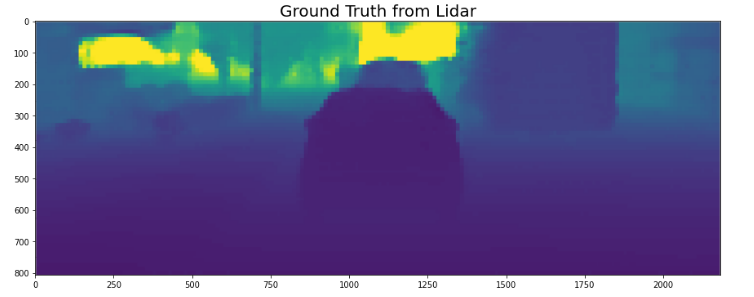
\includegraphics[width=\textwidth]{../imagens/lidar_reference.png}
          \caption{Dados de um LiDAR como referência.}
          \label{fig:lidar_reference}
     \end{subfigure}
     \hfill
     \begin{subfigure}[t]{0.49\textwidth}
          \centering
          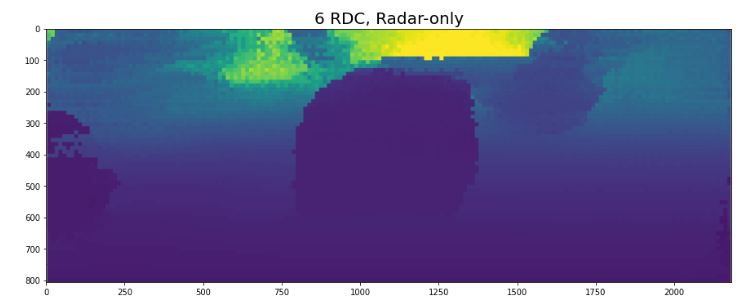
\includegraphics[width=\textwidth]{../imagens/radar_network.png}
          \caption{Exemplo de dados de um radar FMCW após processamento por uma rede neuronal.}
          \label{fig:radar_fmcw_network}
     \end{subfigure}
\end{figure}

\subsection{Laser Rangefinding (LiDAR)}
Operando sob o mesmo princípio físico do radar, mas 
recorrendo a ondas eletromagnéticas de maior frequência 
(como infravermelhos ou luz visível), os sensores LiDAR 
oferecem uma precisão e resolução espacial na ordem dos 
centímetros, permitindo a criação de mapas 3D altamente 
detalhados do ambiente \parencite{serrano2022optimization}. 
Em contrapartida, apresentam um custo superior aos radares 
FMCW e o seu alcance é tipicamente limitado a 300 metros. 
O seu desempenho degrada-se significativamente na presença 
de condições atmosféricas adversas, como chuva, nevoeiro 
ou poeira \parencite{s22197532}, revelando também graves 
dificuldades na deteção de superfícies transparentes ou 
altamente reflexivas \parencite{11155197}, o que impede
a sua utilização para a perceção de ondas oceânicas.

\subsection{Câmaras Óticas}
As câmaras óticas estereoscópicas permitem medir parâmetros das ondas e gerar modelos tridimensionais da superfície do mar. O tempo desta reconstrução 3D depende do algoritmo e hardware; a título de exemplo, a literatura regista tempos de processamento de alguns segundos por modelo, com um erro médio de 10\% na estimativa de amplitude e direção \parencite{app12157447}. 

Além da modelação, estes sensores são valiosos para detetar objetos e distingui-los da ondulação \parencite{jmse12010197}. Contudo, o seu desempenho é severamente condicionado pela iluminação, visibilidade e fenómenos de encandeamento \parencite{sym14071487}. Revelam-se também ineficazes em águas com pouco contraste, onde a ausência de pontos de referência impede a correspondência estéreo necessária para a reconstrução tridimensional. 

Apesar destas limitações geométricas, a visão ótica aliada a modelos de \emph{Deep Learning} tem demonstrado resultados notáveis, permitindo classificar o estado do mar na escala de Beaufort em tempo real e superando as falhas da reconstrução clássica \parencite{11320450}.

\subsection{Radares Marítimos de Banda-X}
Os radares de Banda-X permitem calcular a velocidade e a 
direção das correntes marítimas, possuindo um alcance 
extenso de até 5 km \parencite{rs9121261}. No entanto, 
a sua aplicação em veículos ágeis revela-se pouco prática 
devido ao seu elevado peso, grandes dimensões e considerável 
consumo energético. Acresce o facto de a sua capacidade de 
leitura ser diretamente dependente da ação do vento; 
em condições de vento fraco ou inexistente, este sensor 
perde a capacidade de detetar a ondulação.

\subsection{Sensores Ultrassónicos}
Estes sensores podem ser utilizados para medir a altitude 
em voo estacionário (hovering) ou para detetar obstáculos a 
distâncias muito curtas durante manobras de aproximação e 
aterragem. Apresentam um custo extremamente reduzido, grande 
simplicidade de integração e total imunidade a condições de 
iluminação. Todavia, o seu alcance é muito limitado e falham 
drasticamente quando o veículo se encontra em movimento rápido. São também severamente afetados pela interferência acústica gerada pelos motores do veículo, o que os torna inviáveis para o controlo dinâmico de voo sobre as ondas \parencite{9046805}. Devido a estas limitações, foram descartados para a perceção de ondas oceânicas neste projeto.

\subsection{Câmaras Termográficas (IR)}
As câmaras termográficas, operando tipicamente na banda do infravermelho longo (LWIR - \textit{Long-Wave Infrared}), captam a radiação emitida pelos corpos em função da sua temperatura. Tradicionalmente, no contexto marítimo, estes sensores são vistos como um complemento para a operação contínua, mitigando os efeitos do encandeamento solar e detetando obstáculos (embarcações, fauna marinha) face à assinatura térmica homogénea do fundo oceânico.

No entanto, desenvolvimentos recentes no estado da arte demonstram que a termografia pode assumir um papel primário na própria medição e modelação 3D das ondas. A técnica de estereografia térmica resolve as principais falhas da estereografia ótica convencional. No espetro visível, a superfície da água apresenta propriedades óticas desafiantes para a visão computacional, nomeadamente a elevada transparência, a reflexão especular e a ausência de textura, que dificultam o algoritmo de correspondência (\textit{stereo matching}) \parencite{li2025thermal}. 

No espetro LWIR, pelo contrário, a água comporta-se de forma opaca e apresenta características de imagem consideravelmente mais estáveis e adequadas para a extração de pontos de referência. A combinação de configurações estereográficas térmicas com modelos de \textit{Deep Learning} para a extração de disparidade tem provado ser uma técnica não-contacto altamente eficaz para a medição do campo de ondas e da sua evolução, revelando as câmaras termográficas como um sensor de dupla utilidade: perceção semântica de obstáculos e modelação geométrica da ondulação.

\subsection{Altímetros}
Dada a natureza dos veículos de Efeito de Solo (WIG), que exigem um voo a altitudes extremamente baixas (frequentemente entre 1 a 2 metros) e a altas velocidades, a medição exata e contínua da distância vertical à superfície da água é um requisito de segurança crítico. Enquanto sensores como o LiDAR 3D e o Radar FMCW direcional são utilizados para o mapeamento e modelização espacial da ondulação à frente da plataforma, os altímetros são sensores unidimensionais (1D) dedicados exclusivamente a fechar o ciclo de controlo de altitude.

Para aplicações sobre a água, os altímetros baseados em radares de ondas milimétricas (operando nas bandas dos 60 a 80 GHz) têm-se revelado altamente promissores. Conseguem penetrar o \textit{spray} marítimo e oferecer precisões na ordem dos milímetros a frequências de atualização muito elevadas. A sua integração na arquitetura garante que o veículo mantém o "colchão de ar" necessário para o efeito de solo, ajustando a sua elevação instantaneamente para evitar o impacto com as cristas das ondas que passem sob a sua estrutura.

A Tabela~\ref{tab:sensores} resume e compara as principais capacidades dos sensores
abordados nas secções anteriores, considerando as características mais relevantes
para a perceção de ondas oceânicas a partir de plataformas aéreas.

\begin{table}[H]
\centering
\caption{Comparação das capacidades dos sensores para perceção de ondas oceânicas.}
\label{tab:sensores}
\resizebox{\textwidth}{!}{%
\rowcolors{2}{cloudwhite}{white}
\begin{tabular}{lllllll}
\toprule
\textbf{Sensor} & \textbf{Alcance} & \textbf{Resolução Espacial} & \textbf{Resist.\ Atmosférica} & \textbf{Ind.\ de Iluminação} & \textbf{Medição de Velocidade} & \textbf{Custo Relativo} \\
\midrule
FMCW Radar        & 1-600 m         & Baixa      & Excelente & Sim & Sim (Doppler)  & Moderado    \\
LiDAR             & 1-300 m         & Alta       & Moderada  & Sim & Não            & Elevado     \\
Câmara Ótica      & N/A             & Muito alta & Fraca     & Não & Não            & Baixo       \\
Câmara Termográfica & N/A             & Alta       & Moderada  & Sim & Não            & Moderado    \\
Radar Banda-X     & 1-2000 m        & Baixa      & Boa       & Sim & Sim (Doppler)  & Elevado     \\
Ultrassónico      & 1-10 m          & Moderada   & Boa       & Sim & Não            & Muito baixo \\
\bottomrule
\end{tabular}
}
\end{table}

\parencite{toa2020ultrasonic}
\parencite{rs9121261}

\subsection{Síntese e Escolha das Técnicas de Perceção}
A análise comparativa do estado da arte revela que não existe um sensor único capaz de satisfazer todas as exigências operacionais de um veículo de Efeito de Solo (WIG) em ambiente marítimo. Por conseguinte, a configuração mais apropriada exige uma arquitetura de perceção multissensorial assimétrica e complementar.

Nesta arquitetura, o radar FMCW e as câmaras óticas assumem-se como os sensores primários para a modelação geométrica contínua da superfície oceânica. O radar garante a penetração em condições atmosféricas adversas e a medição cinemática das ondas, enquanto a estereografia compensa a esparsidade e o ruído do radar, permitindo a extração de modelos 3D. Em paralelo, o LiDAR e a câmara termográfica atuarão como os sensores fundamentais para o mapeamento de alta resolução de obstáculos sólidos, e as câmaras óticas garantirão também a avaliação semântica global do estado do mar (Escala de Beaufort).

Adicionalmente, devido ao requisito crítico de voo rasante a alta velocidade, a arquitetura incorpora obrigatoriamente altímetros de ondas milimétricas (1D) para fechar o ciclo de segurança e controlo de altitude. As tecnologias de Banda-X e os ultrassons foram definitivamente descartados devido à sua inadequação ao perfil dinâmico da plataforma.

Por fim, toda a informação exteroceptiva recolhida por esta matriz de sensores carece de referenciação espacial absoluta. Deste modo, a integração de um sistema de navegação inercial (IMU), um Barómetro e um recetor GNSS revela-se estritamente necessária para a estimação da pose do veículo, permitindo a compensação do movimento e o alinhamento geométrico dos dados. É a complexidade metodológica de integrar e sincronizar todas estas fontes de dados díspares que motiva a exploração das técnicas de fusão multissensorial detalhadas no capítulo seguinte.

%%------------------------------- 4. Fusão Multissensorial -------------------

\section{Métodos de Fusão Multissensorial}\label{sec:fusao}

\subsection{Filtro de Kalman}

\subsection{Filtro Complementar}

\subsection{Redes Bayesianas}

\subsection{Dempster-Shafer Reasoning}

\subsection{Deep Learning}
%%------------------------------- 5. Conclusão --------------------------------

\section{Conclusão}\label{sec:conclusao}

%%------------------------------- bibliography --------------------------------

\printbibliography[title={Referências Bibliográficas}]

\end{document}
